\subsection{GraphGPS with HIG and self supervised loss}
\label{sec:graphgps_hig}
GraphGPS is by design a highly malleable model, which allows for easy additions to the code. Thus we decided to implement HIG-GraphClassification in GraphGPS, to combine two already existing papers. For this combination we specifically targeted the Positional Encodings \ref{fig:gps-hig-position}. While implementing HIG, we accidentally created self supervised loss.

\begin{figure}[ht]
    \centering
    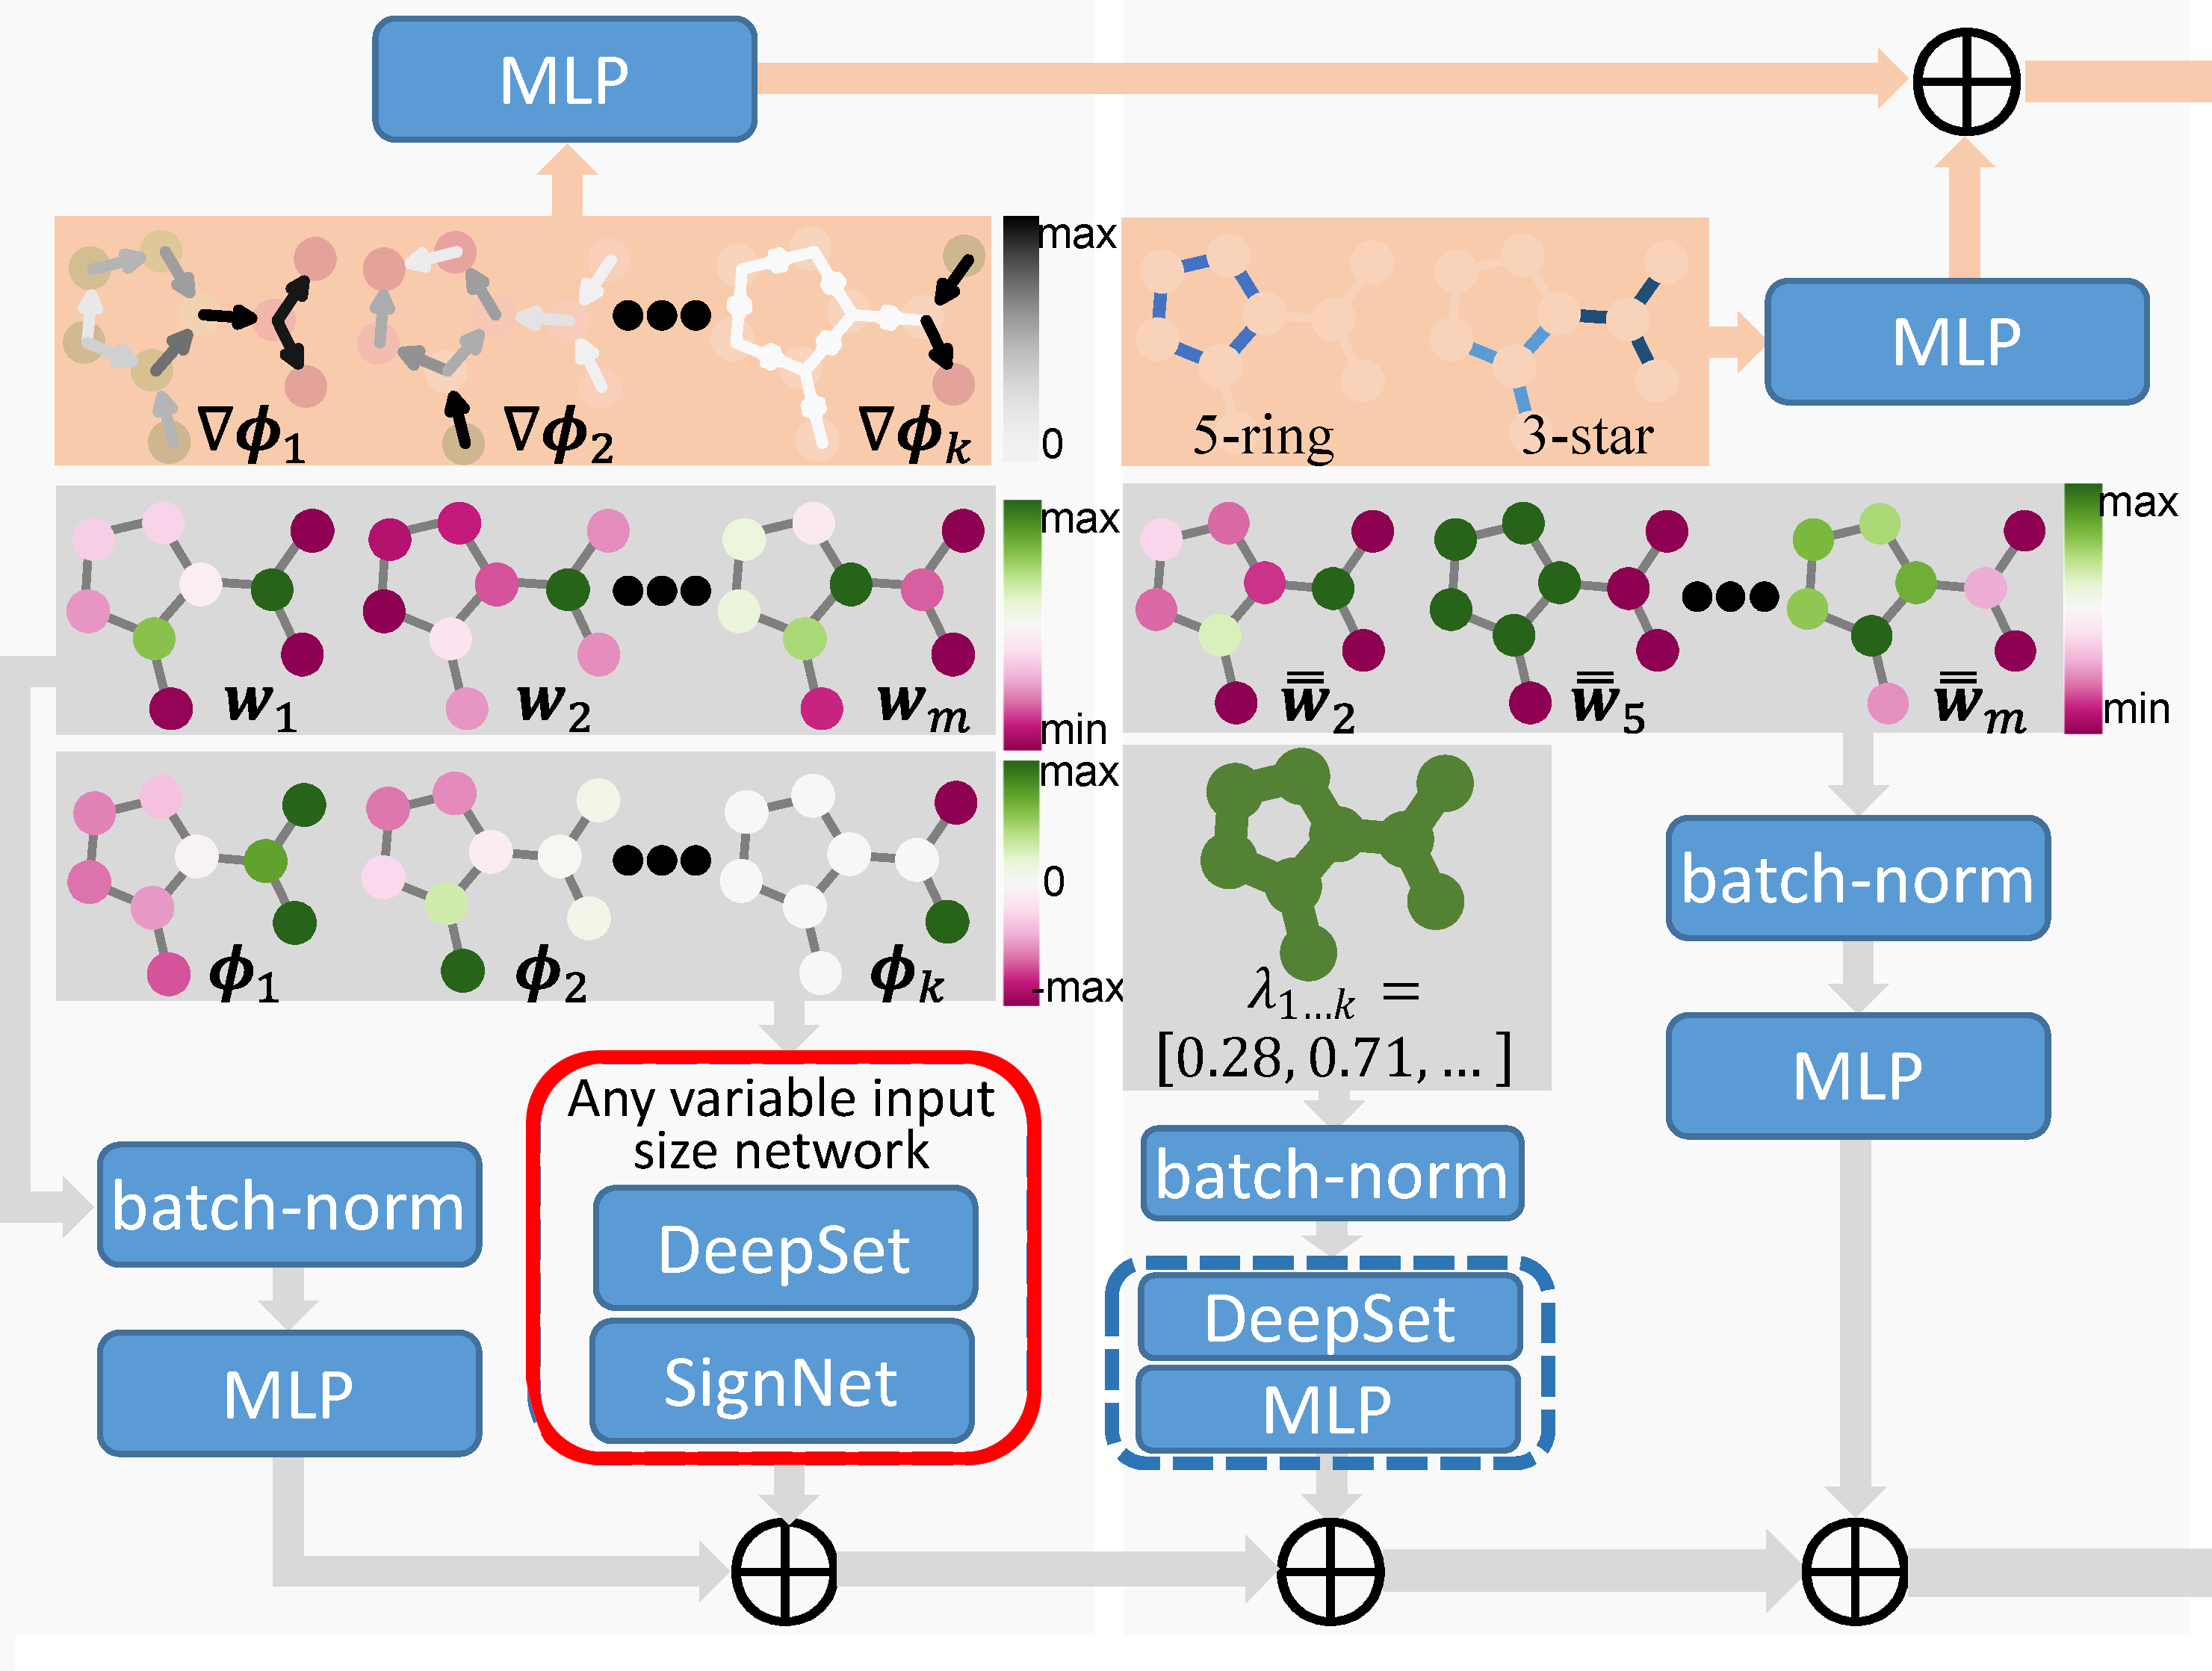
\includegraphics[scale=0.2]{tex/res/gps_hig_position.png}
    \caption{Position of HIG in GraphGPS structure}
    \label{fig:gps-hig-position}
\end{figure}

\subsubsection{Implementation}

The implementation of the heterogeneous Replacement, which involves dropping the feature vector (Table \ref{node_feature_list}) of several randomly selected nodes and replacing them with an interpolated feature mix, can be found in algorithm \ref{algorithm:HiG_Code_in_GraphGPS}. While our implementation does not include the mixing ratio, we have added a Replacement-p parameter and a min\_size parameter. The Replacement-p parameter enables us to specify the probability with which the graph replaces a node with an interpolated feature mix. On the other hand, the min\_size parameter sets a minimum size for the graph. This is because a smaller graph tends to lose more information if a node is replaced, which could be disadvantageous. Additionally, we have included the nodes\_replaced parameter, which allows us to specify the number of nodes that get replaced instead of randomly choosing how many get replaced. \\\\

Previously the if-condition in line 15 was never satisfied, which resulted in a division by 0 in line 27. The values of the Node feature vector are then replaced by very high negative values, e.g. -9223372036854775808. This in combination with how Graphormer \cite{2020graphTransformers} works, resulted in the value getting dropped instead, resulting in a self-supervised loss.

\begin{minipage}{\linewidth}
    \begin{algorithm}[H]
        %\SetKwSty{text}
        \DontPrintSemicolon
        \SetArgSty{text}
        \SetProgSty{text}
        \SetKw{KwIn}{in}
        \SetKw{KwAnd}{and}

        \SetKwProg{Fn}{def}{}{}
        \If{'HiG' in pe\_types}{
            Replacement\_chance = cfg.posenc\_HIG.Replacement\_p\;
            is\_interpolating = np.random.choice(2, 1, p=[1-Replacement\_chance, Replacement\_chance])[0]\;
            minimum\_node\_size = cfg.posenc\_HIG.minimum\_node\_size\;
            nodes\_replaced = cfg.posenc\_HIG.nodes\_replaced\;
            minimum\_node\_size = max(minimum\_node\_size, nodes\_replaced)\;
            \If{data.num\_nodes > minimum\_node\_size \KwAnd is\_interpolating == 1}{
                rand\_ints = np.random.choice(data.num\_nodes, nodes\_replaced\;
                sum = \{\}\;
                \For{rand\_int \KwIn rand\_ints}{
                    data.x[rand\_int] = 0\;
                    sum[rand\_int] = 0\;
                }
                \For{i,j \KwIn zip(data.edge\_index[0], data.edge\_index[1])}{
                    \If{i.item() \KwIn rand\_ints}{
                        \If{j.item() \KwIn rand\_ints}{
                            continue
                        }
                        relevant\_node = j;
                        data.x[i] = torch.add(data.x[i], data.x[relevant\_node])\;
                        sum[i.item()] += 1\;
                    }
                }
                \For{rand\_int \KwIn rand\_ints}{
                    \If{(sum[rand\_int] ==0)}{
                            continue
                        }
                    data.x[rand\_int] = data.x[rand\_int] / sum[rand\_int]
                }
            }
        }
        \caption{HiG-Code in GraphGPS}
        \label{algorithm:HiG_Code_in_GraphGPS}
    \end{algorithm}
\end{minipage}

\subsubsection{Results}
In table \ref{hig_results} are the results of implementing HIG in GraphGPS. The lowest performance is when 5 nodes are replaced by an Replacement. For self supervised loss the Parameter combination of 0.75 Replacement-p, 1 Node Replaced and 20 minimum graph Size performs best. For HIG  this Parameter combination also performs best. HIG outperforms supervised loss, the more nodes are replaced. With the replacement-p going towards 0.5, self supervised loss outperforms HIG.
\begin{table}[ht!]
    \centering
    \caption{Self supervised loss on obgb-molhiv}
    \label{loss_results}
    \begin{tabular}{c || l|l|l|l|}
        Model Focus        & Replacement-p & Nodes Replaced & min.graph size & Test-AUC \\
        \hline
        \hline
        Self supervised loss       & 1.0             & 1                  & 5              & 0.75274  \\
        \hline
        Replacement-p    & 0.5             & 1                  & 5              & 0.77894  \\
                           & 0.1             & 1                  & 5              & 0.77033  \\
                           & 0.01            & 1                  & 5              & 0.7625   \\
        \hline
        Nodes Replaced & 1.0             & 2                  & 5              & 0.73967  \\
                           & 1.0             & 3                  & 5              & 0.73882  \\
                           & 1.0             & 5                  & 10             & 0.71498  \\
        \hline
        min. graph size    & 1.0             & 1                  & 10             & 0.76795  \\
                           & 1.0             & 1                  & 20             & 0.77084  \\
                           & 1.0             & 1                  & 50             & 0.7566   \\
        \hline
        Combination        & 0.5             & 1                  & 20             & 0.77164  \\
                           & 0.75            & 1                  & 20             & 0.78321  \\
    \end{tabular}
\end{table}

\begin{table}[ht!]
    \centering
    \caption{Our HIG-Implementation on obgb-molhiv}
    \label{hig_results}
    \begin{tabular}{c || l|l|l|l|}
        Model Focus        & Replacement-p & Nodes Replaced & min.graph size & Test-AUC \\
        \hline
        \hline
        No HIG             &                 &                    &                & 0.7710   \\
        \hline
        HIG       & 1.0             & 1                  & 5              & 0.77384  \\
        \hline
        Replacement-p    & 0.5             & 1                  & 5              & 0.76834  \\
                           & 0.1             & 1                  & 5              & 0.76564  \\
                           & 0.01            & 1                  & 5              & 0.76275   \\
        \hline
        Nodes Replaced & 1.0             & 2                  & 5              & 0.74348  \\
                           & 1.0             & 3                  & 5              & 0.73382  \\
                           & 1.0             & 5                  & 10             & 0.72977  \\
        \hline
        min. graph size    & 1.0             & 1                  & 10             & 0.76878  \\
                           & 1.0             & 1                  & 20             & 0.76636  \\
                           & 1.0             & 1                  & 50             & 0.78039   \\
        \hline
        Combination        & 0.75            & 1                  & 20             & 0.7792  \\
    \end{tabular}
\end{table}

\subsubsection{Conclusion}
In conclusion, our experiment revealed that the self-supervised loss outperformed our HIG-Implementation, despite the unexpected success given that the code was not intended to function in this way. We believe that this is due to the self-supervised loss being more effective in preventing overfitting. On the other hand, when more nodes are replaced, HIG's performance surpasses that of the self-supervised loss, which may be due to the latter losing too much information at each node. Interestingly, our results also suggest that self-supervised loss on smaller molecules may eliminate crucial information. Further research into supervised loss could shed more light on this phenomenon and offer insights into optimizing molecular representation learning.

